
\chapter{Numerical Methods}
\label{sec:numerics}

\section{Solving equations numerically}
It frequently happens that when confronted with a problem you end up with a mathematical problem or expression that cannot be evaluated analytically. This may be a differential equation that we cannot solve, an integral that has no closed form solution, or even an algebraic equation which does not yield an explicit solution. This is where we have to turn to computer packages or follow a numerical method. Nowadays many computer programs can implement these approaches as standard. However, it is a good idea to understand how to implement a few of these approaches by hand as you may end up writing one of your own at some stage.\\

Chapter 27 of \citep{riley_mathematical_2006}  contains a lot of information about this topic and is a good place to go for more details than we will discuss here.\\

Before moving on to numerical differentiation and integration we will first discuss how to solve algebraic equations numerically. This is all about finding the real roots of an equation $f(x)=0$. This equation can either be algebraic, with $f(x)$ being a polynomial, or transcendental, if $f(x)$ includes trig, log, or exponential terms. We will be using iterative schemes to solve the equations, where we make successive approximations to the true solution, which converge to the true solution. For a method to be successful we need both that the approximations converge to the true solution, and also that we only have a finite number of solutions.\\

It is important to note that different iteration methods will be better at solving certain kinds of problems, in practice some combination of methods is likely to be used. We will see four methods, \textbf{Rearrangement}, \textbf{Linear interpolation}, and \textbf{Bisection}, before discussing \textbf{Newton}'s method, which is the most important method to know in this module. 

\subsection*{Rearrangement}
To explain what we mean by an iterative scheme it is useful to consider the first example method, recasting our equation $f(x)=0$ as
\begin{equation*}
x=\phi(x),
\end{equation*}
for some slowly varying function $\phi(x)$. Our iteration scheme starts from a guess, $x_{0}$ which will not solve $f(x_{0})=0$ but should be picked so that it is close to zero\footnote{It is useful to plot or roughly sketch the function $f(x)$ as then it can be easier to pick a starting point.}. We then have that $x_{1}=\phi(x_{0})$ and can keep repeating this process, i.e. $x_{n+1}=\phi(x_{n})$. The solution we are looking for will be a value of $x$ that is left unchanged by applying $\phi$. \\

The different methods are different ways of building $\phi(x)$ so that we can start the iteration scheme.\\

As an example of how to use the rearrangement iteration consider
\begin{equation}
f(x)=x^{5}-3x^3+2x-4=0.
\label{eq: equation for iterating}
\end{equation}

\begin{figure}[ht]
    \centering
\ThisAltText{Graph of the function that we are studying via iteration.}
 %   \pdftooltip{
    \begin{tikzpicture}[line width=1pt,line cap=round,line join=round, smooth,variable=\x]
     \draw[->] (-0.3,0) -- (6.3,0) node[above] {$x$};
  \draw[->] (0,-4.5) -- (0,3)node[above]{$y$};
 \draw[color=CDnavy, domain=0:5.58]   plot[samples=300] (\x,{(0.33^(5))*\x^(5)-3*(0.33^(3))*\x^(3)+2*(0.33)*\x-4}) node[right] {$f(x)=x^{5}-3x^3+2x-4$};
\filldraw[black] (1.5,0) circle (1pt) node[anchor=north]{$0.5$};
\filldraw[black] (3,0) circle (1pt) node[anchor=north]{$1$};
\filldraw[black] (4.5,0) circle (1pt) node[anchor=north]{$1.5$};
\filldraw[black] (6,0) circle (1pt) node[anchor=north]{$2$};
\filldraw[black] (0,-4) circle (1pt) node[anchor=east]{$-4$};
\filldraw[black] (0,-3) circle (1pt) node[anchor=east]{$-3$};
\filldraw[black] (0,-2) circle (1pt) node[anchor=east]{$-2$};
\filldraw[black] (0,-1) circle (1pt) node[anchor=east]{$-1$};
\filldraw[black] (0,1) circle (1pt) node[anchor=east]{$1$};
\filldraw[black] (0,2) circle (1pt) node[anchor=east]{$2$};
    \end{tikzpicture}
%    }{plots of an exponential and logarithm }
    \caption{A plot of the function $f(x)=x^{5}-3x^3+2x-4$ for $0\leq x\leq 1.86$.}
        \label{fig: interpolation polynomial}
\end{figure}

By rearranging this equation we have that
\begin{equation*}
x=\left(3x^{3}-2x+4\right)^{\frac{1}{5}}.
\end{equation*}
From the plot we in \cref{fig: interpolation polynomial} we see that the root is between $x=1.5$ and $x=2$ and to see how the method works we will not attempt to start from that close to the true root. Here we take $x_{0}=1.8$ and then iterate using 
\begin{equation*}
x_{n+1}=\left(3x_{n}^{3}-2x_{n}+4\right)^{\frac{1}{5}}.
\end{equation*}

The successive values of $x_{n}$ and $f(x_{n})$ are shown in \cref{table:1} and they are closing in on
\begin{equation}
x=1.757632748,
\label{eq: precise root}
\end{equation} 
which is the value of the root to $9$ decimal places. We see from the table that once we got to $x_{5}$ we were only differing from the precise answer in the third decimal places, so are within two parts in $10^{3}$. We can also see that lots of iterations are needed to get an accurate answer. The precise number will depend on the specific problem. \\


\begin{table}[ht]
\centering
\caption{Successive approximations to the root of \cref{eq: equation for iterating} using the rearranged equation. As the convergence is relatively slow we jump several steps at the end to show you it getting closer.}

\vspace{2mm}

\label{table:1}



\begin{tabular}{|c|c|c|} 
 \hline
$n$& $x_{n}$ &$f(x_{n})$\\
 \hline
 $0$ & $1.8$ & $0.99968$ \\
 \hline
$1$ &$1.7805378$ & $0.52247969$ \\
\hline
$2$ &$1.7700175$ & $0.27736234$	\\
\hline
$3$ & $1.7643295$& $0.14849136$\\
\hline
$4$ & $1.761254$& $0.07986324$\\
\hline
$5$ & $1.7595909$ & $0.043059716$\\
\hline
$12$ &$1.75765592$ &$0.00058017842$\\
\hline
$18$ &$1.7576331$& $7.8434818\times10^{-6}$\\
\hline
\end{tabular}
\end{table}

\begin{exercise}
Implement this iteration method numerically  for \cref{eq: equation for iterating} using a programming language or computer program of your choice. I would suggest trying Python or Matlab, but you can use whatever you feel most comfortable with.
\end{exercise}

\subsection*{Linear interpolation}
The next method to look at is \textbf{linear interpolation}.  The idea here is to pick two points $A_{1},B_{1}$ on the graph $y=f(x)$ that lie on either side of the root, i.e. so that $f(A_{1})$ and $f(B_{1})$ have opposite signs. We can then think about the straight line\footnote{This straight line is known as a chord.} joining these points $(A_{1},f(A_{1}))$ to $(B_{1},f(B_{1}))$. An example of this is shown in \cref{fig: interpolation polynomial 2} where $A_{1}=1.5$ and $B_{1}=1.8$.\\

The intersection of this straight line with the $x$-axis is given by
\begin{equation*}
x_{1}=\frac{A_{1}f(B_{1})-B_{1}f(A_{1})}{f(B_{1})-f(A_{1})},
\end{equation*}
We then replace $A_{1}$ or $B_{1}$ by $x_{1}$, find the point on the curve corresponding to $x=x_{1}$ and then iterate this process using the interpolation formula
\begin{equation}
x_{n}=\frac{A_{n}f(B_{n})-B_{n}f(A_{n})}{f(B_{n})-f(A_{n})}.
\label{eq: linear interpolation formula}
\end{equation}


\begin{figure}[ht]
    \centering
\ThisAltText{Graph of the function that we are studying via iteration with the linear regression chord shown.}
 %   \pdftooltip{
    \begin{tikzpicture}[line width=1pt,line cap=round,line join=round, smooth,variable=\x]
     \draw[->] (-0.3,0) -- (6.3,0) node[above] {$x$};
  \draw[->] (0,-4.5) -- (0,3)node[above]{$y$};
 \draw[color=CDnavy, domain=0:5.58]   plot[samples=300] (\x,{(0.33^(5))*\x^(5)-3*(0.33^(3))*\x^(3)+2*(0.33)*\x-4}) node[right] {$f(x)=x^{5}-3x^3+2x-4$};
\filldraw[black] (1.5,0) circle (1pt) node[anchor=north]{$0.5$};
\filldraw[black] (3,0) circle (1pt) node[anchor=north]{$1$};
\filldraw[black] (4.5,0) circle (1pt) node[anchor=north]{$1.5$};
\filldraw[black] (6,0) circle (1pt) node[anchor=north]{$2$};
\filldraw[black] (0,-4) circle (1pt) node[anchor=east]{$-4$};
\filldraw[black] (0,-3) circle (1pt) node[anchor=east]{$-3$};
\filldraw[black] (0,-2) circle (1pt) node[anchor=east]{$-2$};
\filldraw[black] (0,-1) circle (1pt) node[anchor=east]{$-1$};
\filldraw[black] (0,1) circle (1pt) node[anchor=east]{$1$};
\filldraw[black] (0,2) circle (1pt) node[anchor=east]{$2$};
  \draw[color=CDred, -] (4.55,-3.53125) -- (5.45,0.99968 );
  \filldraw[color=CDred] (4.55,-3.53125) circle (1pt) node[anchor=east]{$A_{1}$};
    \filldraw[color=CDred] (5.45,0.99968) circle (1pt) node[anchor=east]{$B_{1}$};
    \end{tikzpicture}
%    }{plots of an exponential and logarithm }
    \caption{A plot of the function $f(x)=x^{5}-3x^3+2x-4$ for $0\leq x\leq 1.86$ with the first linear interpolation chords shown in red.}
        \label{fig: interpolation polynomial 2}
\end{figure}

With each iteration the chord will become shorter and the end points will move until the value of $x_{n}$ converges to the precise value of the root.  The first few steps of this interpolation starting from $A_{1}=1.5$ and $B_{1}=1.8$ are shown in \cref{table:2}.


\begin{table}[ht]
\centering
\caption{Successive approximations to the root of \cref{eq: equation for iterating} using linear interpolation. This is converging very slowly and changes by around $0.0003$ each iteration. }

\vspace{2mm}

\label{table:2}



\begin{tabular}{|c|c|c|c|c|c|c|} 
 \hline
$n$& $A_{n}$ &$f(A_{n})$& $B_{n}$ & $f(B_{n})$& $x_{n}$& $f(x_{n})$\\
 \hline
 $1$ & $1.5$ & $-3.5315$& $1.8$ &$0.99968$& $1.50003$&  $-3.5310$\\
 \hline
 $2$& $1.50003$&$-3.5310$&$1.8$ &$0.99968$& $1.50006$&$-3.53082$\\
 \hline
 $3$& & & & & & \\
 \hline
 $4$& & & & & &\\
 \hline
 $5$& & & & & &\\
 \hline
\end{tabular}
\end{table}


We can see from this example that the linear interpolation method is much slower than rearrangement method, this will not always be true, but is your first hint that you should play around with several approaches before settling on the one that works the best. If you are writing code for these problems, then it is a good idea to have code that can implement any of the iteration schemes that we are discussing here.

\subsection*{Bisection method}

\subsection*{Newton's method}
The main numerical method that is needed in this module is \textbf{Newton's method}, sometimes called the \textbf{Newton-Raphson} method. Newton's method finds the root by constructing the tangent to a curve through the initial point $x_{0}$, and then taking the next point $x_{1}$ to be where the tangent line intersects the $x$-axis.\\

\begin{table}[ht]
\centering
\caption{Successive approximations to the root of \cref{eq: equation for iterating} using Newton's method. For this example, Newton's method converges much quicker than the other methods.}

\vspace{2mm}

\label{table:3}



\begin{tabular}{|c|c|c|} 
 \hline
$n$& $x_{n}$ &$f(x_{n})$\\
 \hline
 $0$ & $1.8$ & $0.99968$ \\
 \hline
$1$ &$1.760530638$ & $0.06382986248$ \\
\hline
$2$ &$1.757647406$ & $0.00032122929$	\\
\hline
$3$ & $1.757632748$& $8.267167839\times10^{-9}$\\
\hline
$4$ & $1.757632748$& $-8.881784197\times10^{-16}$\\
\hline
$5$ & $1.757632748$ & $-8.881784197\times10^{-16}$\\
\hline
\end{tabular}
\end{table}

In other words we start from a guess, $x_{0}$, then construct the tangent line
\begin{equation*}
y(x)=\left(x-x_{0}\right)f'(x_{0})+f(x_{0}).
\end{equation*} 
Once we have the tangent we find the value of $x$ such that $y(x)=0$ and call this $x_{1}$. Doing this for a general point in the iteration $x_{n}$ the iteration scheme is
\begin{equation}
x_{n+1}=x_{n}-\frac{f(x_{n})}{f'(x_{n})}.
\label{eq: Newton iteration scheme}
\end{equation}

An important observation here is that if the points $x_{n}$ get close to a critical point of $f(x)$ then the scheme will break down as then $f'(x_{n})$ will be approaching zero. This means that we need to be very careful about picking our starting point, if we pick one that is on the opposite side of a critical point from a root then we may not be able to get to the root. \Cref{fig: Newton iteration} shows what the first step in Newton's method looks like graphically.\\

%%% This plot is not working very well as zooming in on the polynomial it looks to close a straight line so we cannot see the tangent.
%\begin{figure}[ht]
%    \centering
%\ThisAltText{Graph of the function that we are studying via iteration.}
% %   \pdftooltip{
%    \begin{tikzpicture}[line width=1pt,line cap=round,line join=round, smooth,variable=\x, domain=1.7:1.86, yscale = 1, xscale = 54]
%%     \draw[->] (4.2,0) -- (6.3,0) node[above] {$x$};
%%  \draw[->] (4.2,-4.2) -- (4.2,3)node[above]{$y$};
%% \draw[color=CDnavy, domain=4.2:5.58]   plot[samples=300] (\x,{(0.33^(5))*\x^(5)-3*(0.33^(3))*\x^(3)+2*(0.33)*\x-4}) node[right] {$f(x)=x^{5}-3x^3+2x-4$};
%%%\filldraw[black] (1.5,0) circle (1pt) node[anchor=north]{$0.5$};
%%%\filldraw[black] (3,0) circle (1pt) node[anchor=north]{$1$};
%%\filldraw[black] (4.5,0) circle (1pt) node[anchor=north]{$1.5$};
%%\filldraw[black] (6,0) circle (1pt) node[anchor=north]{$2$};
%%\filldraw[black] (4.2,-4) circle (1pt) node[anchor=east]{$-4$};
%%\filldraw[black] (4.2,-3) circle (1pt) node[anchor=east]{$-3$};
%%\filldraw[black] (4.2,-2) circle (1pt) node[anchor=east]{$-2$};
%%\filldraw[black] (4.2,-1) circle (1pt) node[anchor=east]{$-1$};
%%\filldraw[black] (4.2,1) circle (1pt) node[anchor=east]{$1$};
%%\filldraw[black] (4.2,2) circle (1pt) node[anchor=east]{$2$};
%
%% draw axes
%\draw [->] (1.7,0) -- (1.9,0) 	node [anchor=west]		{$x$};
%\draw [->] (1.7,-3) -- (1.7,3) 	node [anchor=south]	{$y$};
%
%% x-axis tick marks
%\foreach \x in {1.75, 1.80, 1.85}
%	\draw (\x, 3pt) -- (\x,-3pt) node [anchor=north] {$\x$};
%	
%% y-axis tick marks
%%\draw (1.6,-4)--(1.6,-4)node [anchor=east] {$-4$};
%\draw (1.7,-3)--(1.7,-3)node [anchor=east] {$-3$};
%\draw (1.7,-2)--(1.7,-2)node [anchor=east] {$-2$};
%\draw (1.7,-1)--(1.7,-1)node [anchor=east] {$-1$};
%\draw (1.7,1)--(1.7,1)node [anchor=east] {$1$};
%\draw (1.7,2)--(1.7,2)node [anchor=east] {$-2$};
%
%%Newton's method lines
%\draw (1.8,3pt)--(1.8,-3pt)node [anchor=south] {$x_{0}$};
%\draw[dotted] (1.8,0) -- (1.8,0.99968);
%\draw[color = CDred] (1.8,0.99968)--(1.76,0) node[anchor = south]{$x_{1}$};
%
%    % draw function
%    \draw[color=CDnavy] plot (\x,{\x^(5)-3*\x^(3)+2*\x-4});
%    \end{tikzpicture}
%%    }{plots of an exponential and logarithm }
%    \caption{A zoomed in plot of the function $f(x)=x^{5}-3x^3+2x-4$  showing the first step of Newton's method, after one step, the result is already so close that we cannot see the other steps if they are plotted.}
%        \label{fig: interpolation polynomial zoomed}
%\end{figure}

\begin{figure}[ht]
    \centering
    %\pdftooltip{
    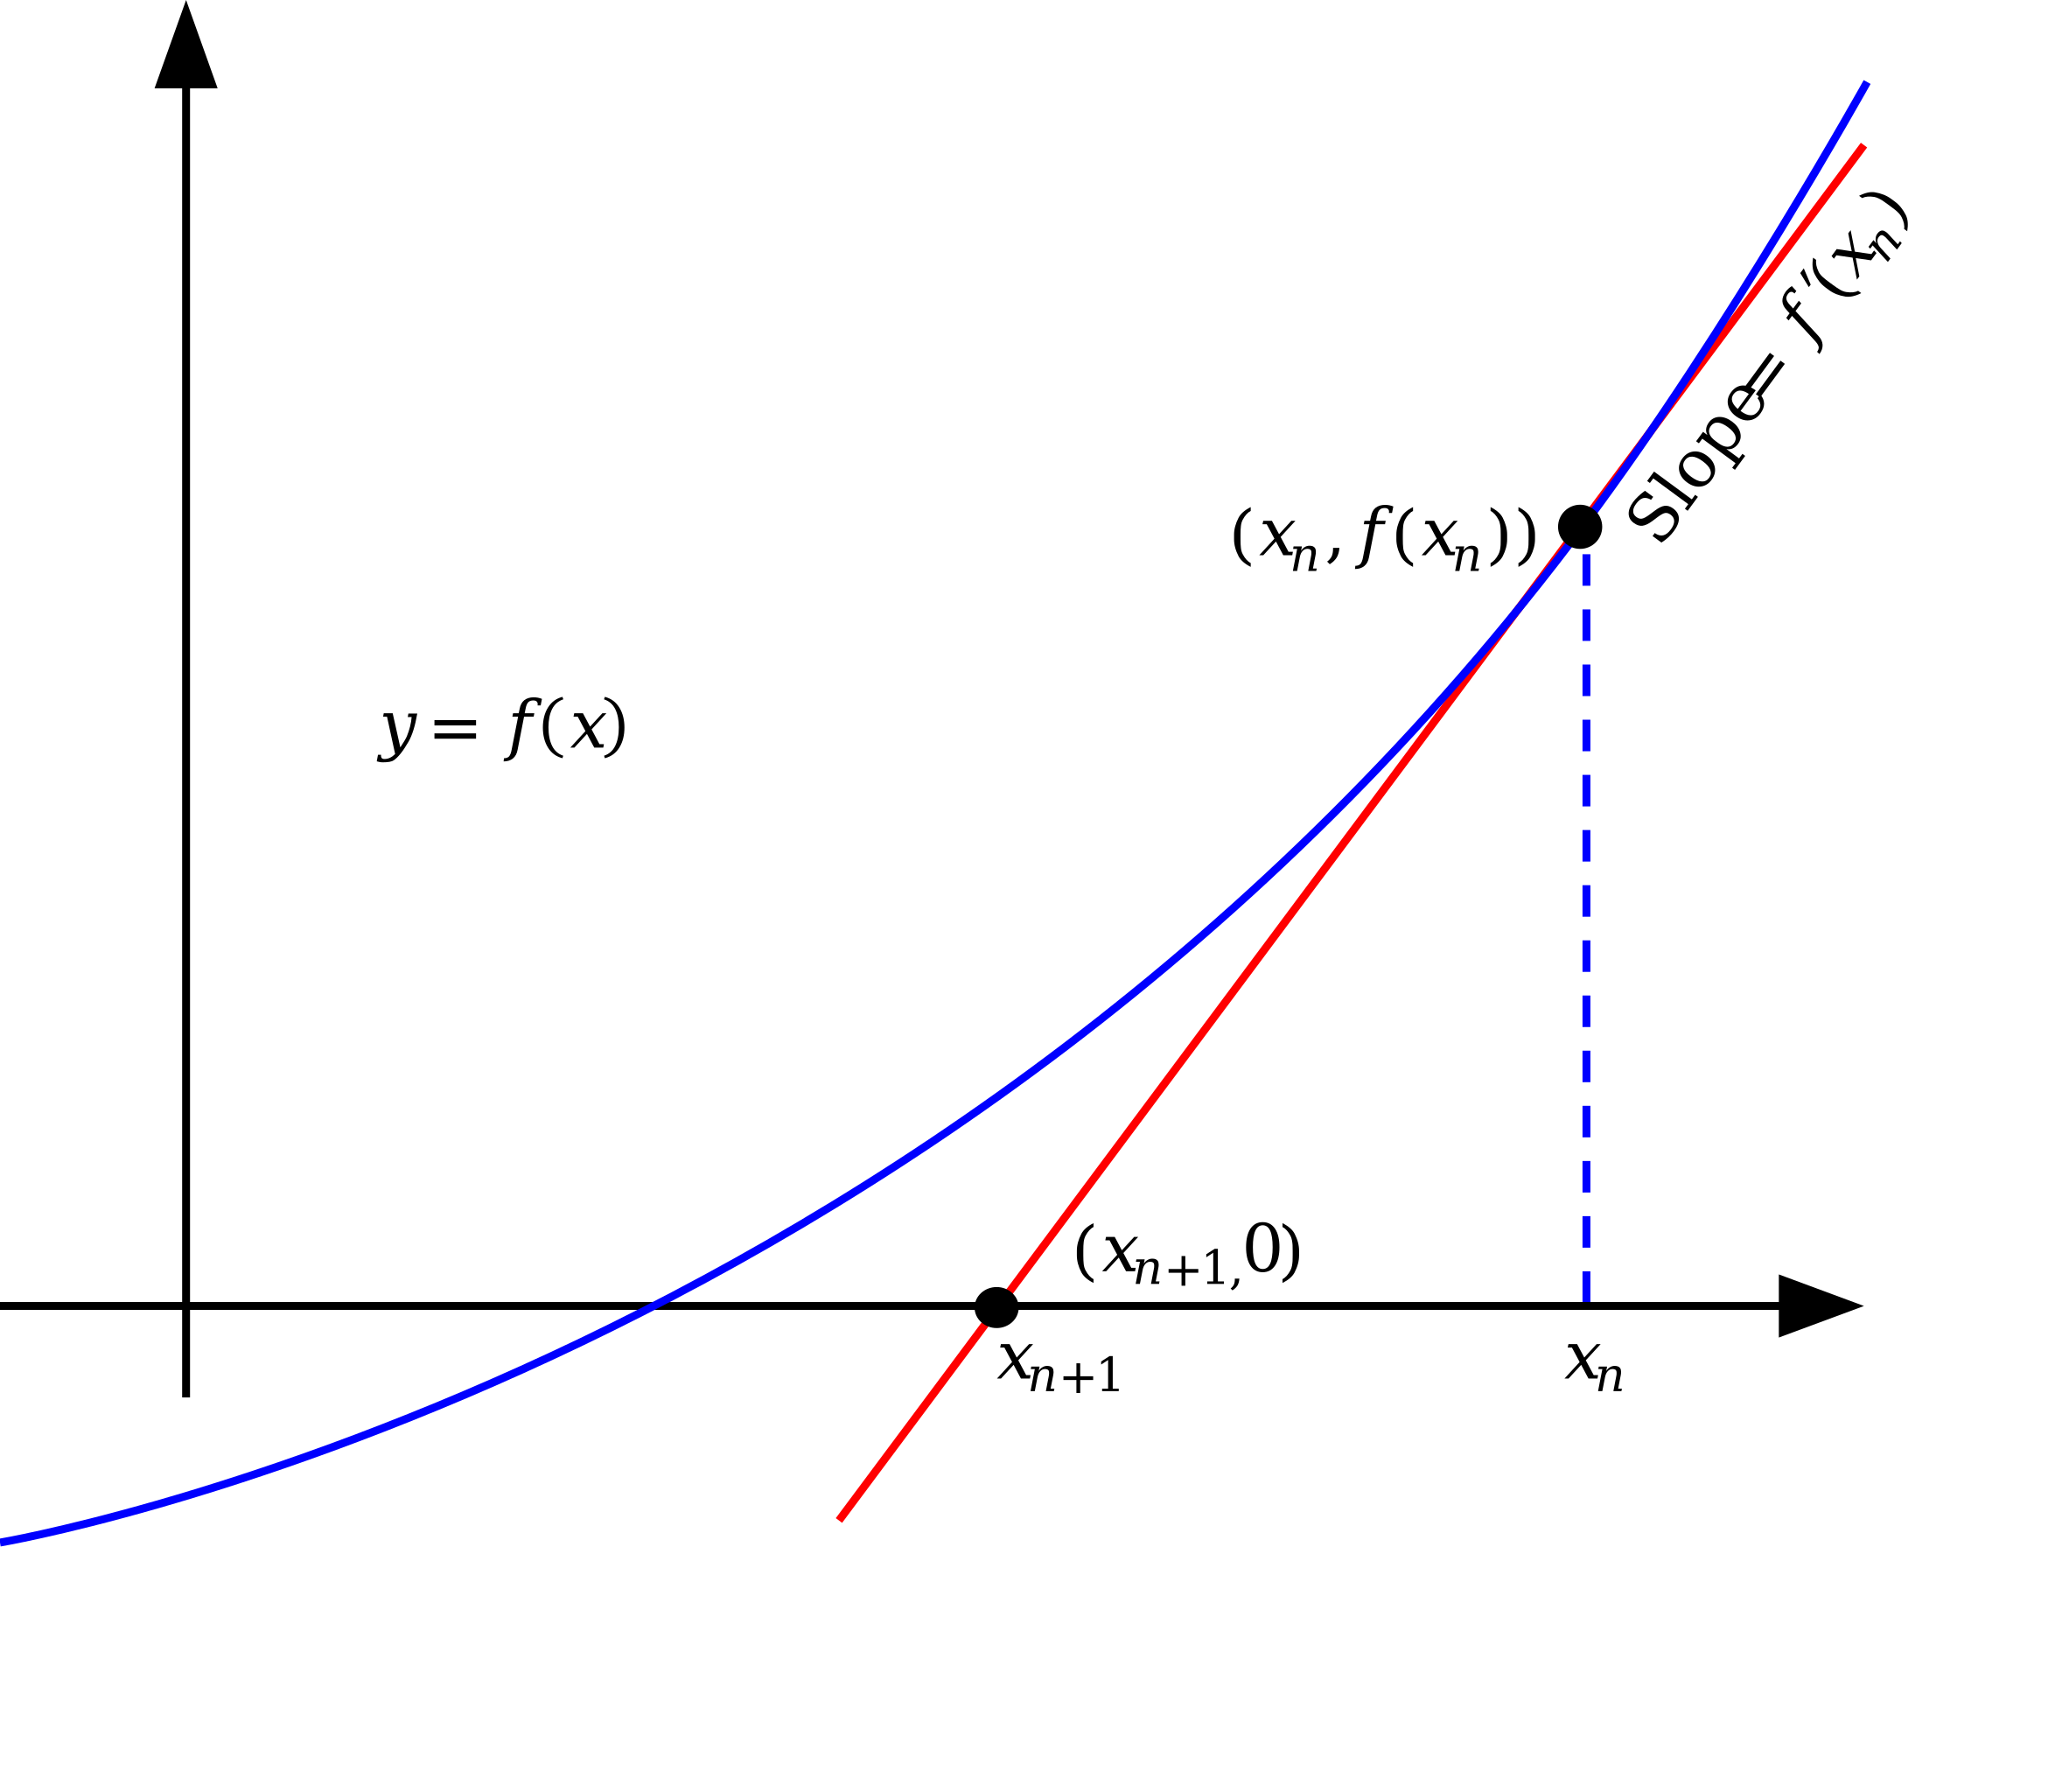
\includegraphics[width=0.5\textwidth, alt ={A schematic of the first step of Newton's method for finding roots}]{figures/Newton_iteration}
    %}{A schematic of a derivative as a tangent to a curve. }
    \caption{The first step of Newton's iteration method to find the root of $f(x)$. We pick a point $x_{0}$ then find the tangent to $f(x)$ at $x_{0}$ and solve for the point $x_{1}$ where this tangent intersects the $x$-axis. This is repeated until we converge on the root.}
\label{fig: Newton iteration}
\end{figure}


For the specific equation in \cref{eq: equation for iterating} we have that
\begin{equation}
x_{n+1}=x_{n}-\frac{x_{n}^{5}-3x_{n}^3+2x_{n}-4}{5x_{n}^{4}-9x_{n}^{2}+2}.
\end{equation}

Starting from $x_{0}=1.8$ we get the sequence in \cref{table:3}. This iteration scheme converges to the precise answer of \cref{eq: precise root} much quicker than the other methods.


Newton's method is the approach that you need to be able to use during this module so we will treat a couple more examples using it. There are a couple more examples on \citep{calcI} if you want to see more.

\begin{ex}
Use Newton's method to determine an approximation to the solution to $\sin{x} = -x$ that lie in the interval $[-1,1]$. Find the approximation to $6$ decimal places.\\

First we need to pick a starting point $x_{0}$. Here we will take $x_{0}=0.5$, you can get an idea of what value to pick by plotting the function. For this example we have that
\begin{equation}
f(x)=\sin(x)+x=0,
\label{eq: sin +x roots}
\end{equation}
so the iteration equation for Newton's method \cref{eq: Newton iteration scheme} becomes
\begin{equation*}
x_{n+1}=x_{n}-\frac{\sin{x_{n}}+x_{n}}{\cos{x_{n}}+1}.
\end{equation*}

The first approximation is then
\begin{equation*}
x_{1}=\frac{1}{2}-\frac{\sin{\frac{1}{2}}+\frac{1}{2}}{\cos{\frac{1}{2}}+1}=-0.0216418
\end{equation*}

\begin{table}[ht]
\centering
\caption{Successive approximations to the root of \cref{eq: sin +x roots} using Newton's method.}

\vspace{2mm}

\label{table:4}



\begin{tabular}{|c|c|c|} 
 \hline
$n$& $x_{n}$ &$f(x_{n})$\\
 \hline
 $0$ & $0.5$ & $0.979426$ \\
 \hline
$1$ &$-0.021642$ & $-0.043282$ \\
\hline
$2$ &$2\times10^{-6}$ & $3.\times10^{-6}$	\\
\hline
$3$ & $0$& $0$\\
\hline
\end{tabular}
\end{table}

The further iteration steps are shown in \cref{table:4}, and we see that to 6 decimal places, it only takes $4$ iterative steps to find that the root is at $x=0$. If we did any more steps we would see that these remain at $x=0$.

\end{ex}

Now we can consider one of the examples from \citep{calcI} which shows when Newton's method does not work.

\begin{ex}
Starting from $x_{0}=1$ we will apply Newton's method to $\sqrt[3]{x}$.\\

Intuitively it is clear that the root is $x=0$. However, Newton's method will not find this root. For this example \cref{eq: Newton iteration scheme} becomes
\begin{equation*}
x_{n+1}=x_{n}-\frac{\sqrt[3]{x}}{\frac{1}{3}x^{-\frac{2}{3}}}=x_{n}-3x_{n}=-2x_{n}.
\end{equation*}

This already tells us that instead of converging to $x=0$, Newton's method will diverge with $x_{1}=-2$, $x_{2}=4$, $x_{3}=-8$, $x_{4}=16$, \dots{}. This is the opposite of what we want. Fortunately, it became obvious quite quickly that the method was not working and we did not have to waste much time before discovering that we needed to used a different model.
\end{ex}

\begin{exercise}
Write a computer program to implement Newton's method and use it to find the roots in the examples above, where Newton's method works.
\end{exercise}

\subsection*{Secant method}
A variant of Newton's method is the \textbf{Secant} method, where we start with two estimates of the root, $x_{0}$ and $x_{1}$ and estimate the derivative as being the Newton quotient
\begin{equation*}
Q(x_{0},x_{1})=\frac{f(x_{1})-f(x_{1})}{x_{1}-x_{0}},
\end{equation*}
so that
\begin{equation*}
x_{2}=x_{1}-\frac{f(x_{1})}{Q(x_{0},x_{1})}=x_{1}-\frac{f(x_{1})}{\frac{f(x_{1})-f(x_{1})}{x_{1}-x_{0}}}.
\end{equation*}

This means that the iteration scheme is given by
\begin{equation}
x_{n+1}=x_{n}-\frac{f(x_{n})}{Q(x_{n-1},x_{n})}=x_{n}-\frac{f(x_{n})}{\frac{f(x_{n})-f(x_{n-1})}{x_{n}-x_{n-1}}}
\label{eq: secant method}
\end{equation}

Geometrically, the secant method can also be viewed as constructing a line nearby our function and moving to the point where this line cuts the $x$-axis. However, this line is no longer a tangent line, but is a secant. 

\begin{ex}
For 
\begin{equation*}
f(x)=x^{2}-10,
\end{equation*}
and taking $x_{0}=2$, $x_{1}=3$ we find $x_{2}$ using the secant method as follows:

\begin{align*}
x_{2}&=x_{1}-\frac{f(x_{1})}{\frac{f(x_{1})-f(x_{0})}{x_{1}-x_{0}}}\\
	&=3-\frac{-1}{\frac{-1-(-6)}{3-2}}\\
	&=3+\frac{1}{7}\\
	&=3.14286.
\end{align*}
This is an equation that we can solve directly by the rearrangement method since $f(x)=0$ corresponds to $x^{2}=10$ so the exact answers are $x=-\sqrt{10}\simeq -3.16228$ and $x=\sqrt{10}\simeq 3.16228$. We can see that $x_{2}$ is already approaching this exact answer.

\end{ex}

\subsection*{Convergence and errors}
The absolute error of a numerical method is the difference between the true solution $x$ and the approximate solution $\xi$, $\epsilon =\vert x-\xi\vert$. It can be hard to estimate the absolute error unless we already know the exact solution. \\

We say that an iteration scheme converges when it subsequent iterations do not change the value of $x_{n}$, at least to the accuracy that we are looking for. Not every method will converge for a given problem, We have already seen that Newton's method does not converge for the cube root, $\sqrt[3]{x}$. You will gain experience of which methods works best for which type of of problem. In this module, you will mainly be using Newton's method so you need to remember that it can fail.

\section{Numerical differentiation}

\section{Numerical integration}

\section{Numerical approaches to differential equations}